\chapter{Experiments}

After providing an overview of the game of Durak and introducing the agents under consideration, we will now proceed to conduct experiments to determine which of these agents is strongest. We will conduct experiments in both open and closed world environments. Through these experiments, we will gain a better understanding of the adaptability and effectiveness of the agents in both environments, and determine whether the agents that performed best in perfect information scenarios are able to achieve similar success in an imperfect one.

To conduct our experiments, we will use the \texttt{-tournament} parameter available in the command line interface (as described in Section \ref{CLI}). This option lets us configure the participating AI agents and their respective parameters, as well as the environment for the tournament. In order to compare the agents in both open and closed world scenarios, we will present the results of these experiments in separate sections. The tournament will consist of full games with trump cards, and so the respective parameters \texttt{-include\_trumps} and \texttt{-start\_rank=6} will be set accordingly. In order to strike a balance between accuracy and efficiency, we will set the \texttt{-total\_games} parameter to 500. This number of games may allows us to identify the strongest and weakest agents with a sufficient level of confidence, while not unduly prolonging the experiment. However, as previously mentioned in Section \ref{CLI}, if the total number of games is not sufficient to confidently determine the winner, the program will increment the total number of games by 500 until the maximum number of games, 10 000, is reached. This process ensures that we are able to accurately identify the top performing AI agent while still minimizing the overall length of the experiment.

\section{Open world}

With the game environment parameters set to be  in the perfect information world, we will proceed to configure the parameters for the various agents. Some agents, such as Random, Greedy, and Smart, do not require any additional parameters as their strategies are simple and do not involve game tree search. However, Minimax and MCTS, as described in Sections \ref{minimax} and \ref{MCTS} respectively, do require the configuration of certain parameters in order to perform at their best. In order to determine the optimal values for these parameters, we will run a set of games to identify the values that best suit the tournament environment before comparing with other agents. It is important to note that the selected parameters should result in an average move time of around 100ms in order to identify the most efficient configuration for the agent.

\subsection{Configuring Minimax Parameters}

In order to optimize the performance of the Minimax agent in an open world environment, we must determine the optimal values for the \texttt{depth} and \texttt{eval} parameters. We will use the playout heuristic for the \texttt{eval} parameter as it is generally superior to the basic heuristic. To find the best value for the \texttt{depth} parameter, I ran a 1000 game experiment that tries different values for it against the Greedy agent. 

\begin{figure}[h]
  \centering
  \captionsetup{justification=centering}
  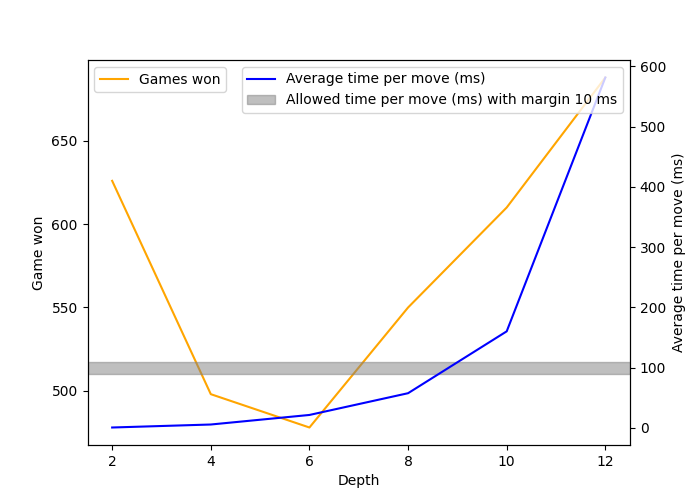
\includegraphics[width=0.8\textwidth]{../img/minimax_config_openworld.png}
  \caption{Comparison of number of wins of different fixed depths parameters in Minimax agent along with average time taken per ply in the open world}
  \label{minimaxOWDepth}
\end{figure}

Figure \ref{minimaxOWDepth} illustrates the number of games won and the average time taken per ply by the Minimax agent with different depth parameters. The plot shows that the number of games won by the Minimax agent improves as the depth of the game tree exploration increases. The same trend can be observed for the average time taken to make a move. However, it is surprising to see that lower depth values such as 2 and 3 have a higher number of games won than the highest depth value of 6, which has the lowest number of wins. This observation warrants further investigation. Besides this, a horizontal shaded line is included in the plot to represent the optimal average time that the agent should take to make a move. It can be observed that the grey shaded line intersects with the average time of the Minimax agent at a depth of 9. This suggests that, in an open environment, this value of the parameter is the most suitable and will be used in the tournament.

Figure \ref{minimaxOWEval} illustrates the comparison between two heuristic evaluation functions, namely \texttt{basic} and \texttt{playout}, for the Minimax agent with a fixed depth of 9. The left subplot shows the number of games won for the two evaluation functions, and the right subplot displays the average time (ms) taken to make a move. It can be observed that the playout heuristic outperforms the basic heuristic in terms of number of games won, achieving almost twice the number of wins of the basic heuristic. However, the playout heuristic is slower than the basic heuristic, as shown by the right subplot. Despite this, the playout heuristic still performs around the optimal time range of 100ms, making it the preferred choice for the tournament. As a result, the Minimax agent will use the depth 9 and playout heuristic for the tournament.

\begin{figure}[h]
  \centering
  \captionsetup{justification=centering}
  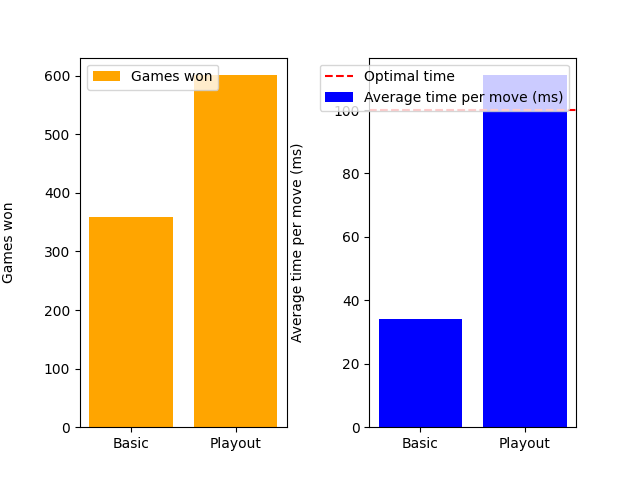
\includegraphics[width=0.8\textwidth]{../img/minimax_eval_openworld.png}
  \caption{Comparison of number of wins and average time taken per ply of \texttt{basic} and \texttt{playout} evaluation functions in Minimax agent in the open world}
  \label{minimaxOWEval}
\end{figure}

\subsection{Configuring MCTS Parameters}

In order to compare MCTS agents with other agents in the open world, it is necessary to determine the optimal values for the parameters \texttt{limit}, \texttt{c}, and \texttt{simulation}. To begin, the exploration constant was set to 1.41, which is typically an optimal value \citep{AI4Ed}, and the \texttt{simulation} was set to \texttt{greedy}. With these parameters in place, an experiment was conducted using 1000 games to find the value of \texttt{limit} by trying various values of iterations to identify the optimal value. The results of this experiment are depicted in Figure \ref{mctsOWIterations}.

\begin{figure}[h!]
  \centering
  \captionsetup{justification=centering}
  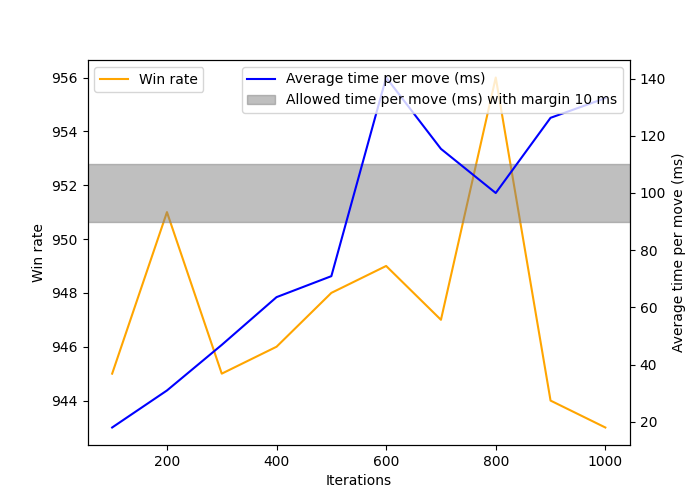
\includegraphics[width=0.8\textwidth]{../img/mcts_iterations_openworld.png}
  \caption{Comparison of win rates and average time taken per ply of different fixed iterations in MCTS algorithm in the open world}
  \label{mctsOWIterations}
\end{figure}

Similar to the Minimax agent, it can be seen that an increase in the number of \texttt{iterations} generally results in a corresponding increase in the average time taken per move, as well as an increase in the win rate. By examining the shaded region in Figure \ref{mctsOWIterations}, which represents the optimal time per move, it can be determined that the optimal value for the \texttt{iterations} parameter is 800. This value results in a relatively high win rate and the lowest average time taken per move.

With the \texttt{iterations} parameter set to 800 and the \texttt{simulation} value remaining at greedy, a new experiment was conducted to determine the optimal value for the \texttt{c} exploration parameter in MCTS. The results of this experiment are shown in Figure \ref{mctsOWC}. From the figure, it can be observed that the optimal value for the \texttt{c} parameter is 1.00, as it yields the highest number of wins while still operating within the optimal average time per move.

\begin{figure}[h!]
  \centering
  \captionsetup{justification=centering}
  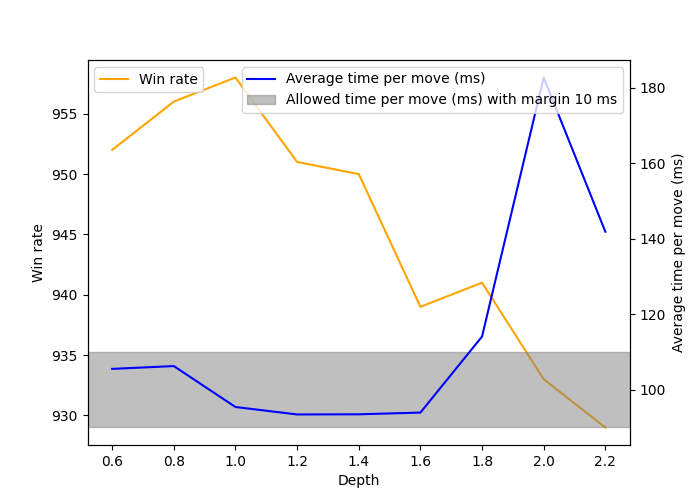
\includegraphics[width=0.8\textwidth]{../img/mcts_c_openworld.png}
  \caption{Comparison of number of wins and average time taken per ply of different fixed exploration parameters in MCTS algorithm in the open world}
  \label{mctsOWC}
\end{figure}

Like in the comparison of heuristic evaluation functions for the Minimax agent, bar plots were used to visualize the number of games won and average times per move for different simulation types in the MCTS algorithm. The left subplot in Figure \ref{mctsOWSimulations} compares the number of games won of the two simulations, and it can be seen that the greedy simulation performs significantly better than the random playouts. Additionally, the greedy simulation is much faster than the random playouts, as can be seen in the right subplot. This is due to the nature of random simulation, as discussed in Section \ref{MCTS}. Based on these results, we can conclude that the optimal parameters for the simulation in MCTS are greedy.

\begin{figure}[h]
  \centering
  \captionsetup{justification=centering}
  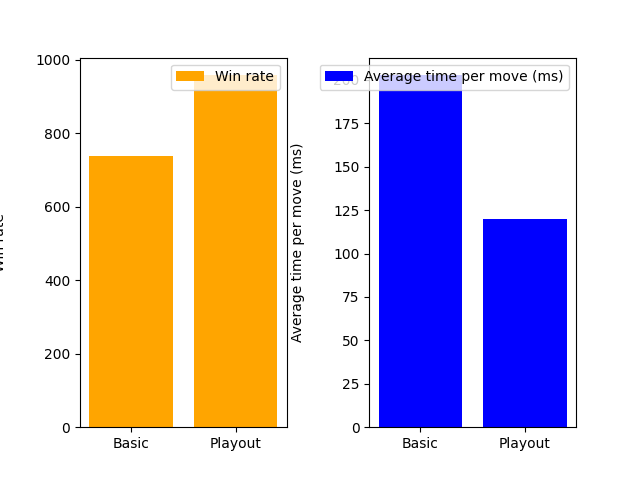
\includegraphics[width=0.8\textwidth]{../img/mcts_simulation_openworld.png}
  \caption{Comparison of number of games won and average time taken per ply of \texttt{random} and \texttt{greedy} simulations in MCTS algorithm in the open world}
  \label{mctsOWSimulations}
\end{figure}

\subsection{Tournament}
In order to begin the tournament, the following list of agents and their corresponding parameters were used: Random, Greedy, Smart, Minimax (depth 9 and playout heuristic evaluation function), and MCTS (limit 800, exploration parameter 1.00 and greedy simulation type).

Furthermore, the game environment was configured with the following settings: open world, including trumps, 500 games and starting rank 6.

The tournament was initiated using the following command, with the aforementioned configurations.

\begin{lstlisting}
$ dotnet run -tournament="random/greedy/smart/minimax:depth=9,eval=playout/mcts:limit=800,c=1.00,simulation=greedy" -total_games=500 -open_world
\end{lstlisting}

It is important to note that \texttt{-include\_trumps} and \texttt{=start\_rank=6} game environment parameters are not explicitly listed in the above command as they are already set to their default values in the game setup.

To improve the readability of the table of tournament results, we will use shortened versions of the long agent names as aliases. The full names and their corresponding aliases are listed below:

\begin{itemize}
	\item \textbf{minimax} := minimax:depth=9:eval=playout
	\item \textbf{mcts} := mcts:limit=800:c=1.00:simulation=greedy
\end{itemize}

\begin{table}[]
\captionsetup{justification=centering}
\begin{tabularx}{\textwidth}{|X|X|X|X|X|X|}
\toprule

                                        & random               & greedy               & smart                & minimax & mcts \\ \midrule
random                                  &                      & \footnotesize{5.6\%-11.3\% (500)}   & \footnotesize{3.3\%-8.0\% (500)}    & \footnotesize{1.2\%-4.6\% (500)}            & \footnotesize{0.0\%-1.1\% (500)}                       \\ \midrule
greedy                                  & \footnotesize{88.7\%-94.4\% (500)}  &                      & \footnotesize{45.7\%-49.9\% (3500)} & \footnotesize{33.5\%-43.6\% (500)}          & \footnotesize{1.1\%-4.4\% (500)}                       \\ \midrule
smart                                   & \footnotesize{92.0\%-96.7\% (500)}  & \footnotesize{50.1\%-54.3\% (3500)} &                      & \footnotesize{34.7\%-45.0\% (500)}          & \footnotesize{2.8\%-7.2\% (500)}                       \\ \midrule
minimax            & \footnotesize{95.4\%-98.8\% (500)}  & \footnotesize{56.4\%-66.5\% (500)}  & \footnotesize{55.0\%-65.3\% (500)}  &                              & \footnotesize{16.4\%-24.8\% (500)}                     \\ \midrule
mcts & \footnotesize{98.9\%-100.0\% (500)} & \footnotesize{95.6\%-98.9\% (500)}  & \footnotesize{92.8\%-97.2\% (500)}  & \footnotesize{75.2\%-83.6\% (500)}          &                                         \\ \bottomrule
\end{tabularx}
    \caption{Tournament between the agents in the open world}
    \label{tournamentOpenWorld}
\end{table}

It should be noted that in this tournament, every pair of agents mentioned in the command line played against each other to determine the winner. These agents did not play against themselves, as this would provide almost the same win rate and the tournament would continue to increase the number of games played for them.

From the Table \ref{tournamentOpenWorld}, the results of the tournament indicate that the MCTS agent with the parameter configuration of \texttt{simulation=greedy}, \texttt{limit=800} and \texttt{c=1.00}  was the clear winner, with a consistently high win rate against all other opponents. In particular, the MCTS agent outperformed the other agents, with win rates of 98.9\%-100.0\% against Random, 95.6\%-98.9\% against Greedy, and 92.8\%-97.2\% against Smart. Due to the dominance of the MCTS algorithm, all results were gathered after 500 games, with no need for additional increments.

The Minimax agent performed performed well against the Random, Greedy and Smart agents, although its results were not as strong as those of the MCTS agent. However, 500 games were sufficient to identify the clear winner in these matchups. 

In summary, the MCTS agent with the specified parameter configuration emerged as the clear winner in terms of win rate, with a strong performance against all other agents. The Minimax agent with the specified parameter configuration came in second, with strong performances against the random, greedy, and smart agents. The smart agent came in third, with a win rate that outperformed the greedy agent, although it took 3500 simulations to find a significant winner between the two. The greedy agent came in fourth, while the random agent had the lowest win rate among all agents. Overall, these results indicate that the MCTS and Minimax agents with their respective parameter configurations are the most effective at winning games, while also having good performance in terms of average time per move.

\section{Closed world}

While the open world setting provides a useful reference point for evaluating the performance of different agents, it is also important to consider how they perform in a closed world environment. As previously mentioned, the normal game of Durak is played in a closed world, with players only able to see their own cards and the trump card that is face up. In this section, we will examine the performance of various agents in a closed world setting and compare it to their performance in the open world. Similar to the open world setting, it is necessary to configure the parameters for Minimax and MCTS agents in a closed world environment in order to optimize their performance. This configuration process includes setting the value of the additional \texttt{samples} parameter to find the frequent move in the hidden state (details in Section \ref{closedWorld}. To determine the optimal values for all relevant parameters, a series of games will be conducted to identify the values that are most suitable for the tournament environment just like before. It is important to ensure that the selected parameters result in an average move time of around 100ms in order to identify the most efficient configuration for the agent.

\subsection{Configuring Minimax Parameters}

In order to optimize the performance of the Minimax agent in an closed world environment, we must determine the optimal values for the \texttt{depth}, \texttt{eval} and \texttt{samples} parameters. We will use the playout heuristic for the \texttt{eval} parameter as it is generally superior to the basic heuristic and set the value 10 to the \texttt{samples} parameter, as this value allows for a faster search process while still providing sufficient information to identify the most frequent move. To find the best value for the \texttt{depth} parameter, I ran a 100 game experiment that tries different values for it against the Greedy agent. The decrease in the number of games can be attributed to the fact that searching for optimal moves using strategies like Minimax and MCTS becomes slower in a closed world environment. This is because these strategies require sampling the game state a specific number of times, the value of \texttt{samples}, in order to determine the most frequent move, which can be time-consuming.

\begin{figure}[h]
  \centering
  \captionsetup{justification=centering}
  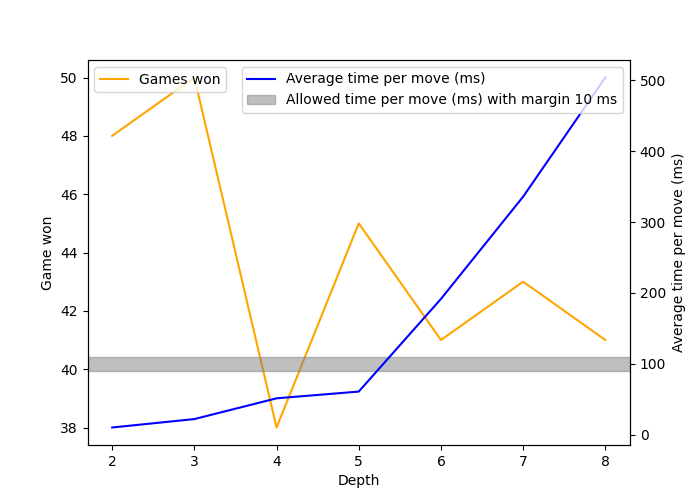
\includegraphics[width=0.8\textwidth]{../img/minimax_depth_closedworld.png}
  \caption{Comparison of number of games won of different fixed depths parameters in Minimax agent along with average time taken per ply in the closed world}
  \label{minimaxCWDepth}
\end{figure}

Figure \ref{minimaxCWDepth} illustrates the number of games won and the average time taken per ply by the Minimax agent with different depth parameters in the closed world. Unlike the open world, the plot shows that the number of games won by the Minimax agent does not improve as the depth of the game tree exploration increases. One potential reason for the lack of an increase in the win rate as the depth increases is that the value of the samples is not large enough. This may prevent the search process from considering all possible moves, leading to the selection of suboptimal moves. The average time taken to make a move, on the other hand, does follow the trend just like the open world: takes more time to make a move as the depth increases. It is unexpected to see that the number of games won fluctuates as the value of the depth parameter increases. This phenomenon warrants further investigation to understand the underlying cause. It can be observed that the highest number of games won is achieved when the depth parameter is set to 3. In addition to providing the best results, this setting also results in relatively fast move times. This suggests that, in the closed environment, this value of the parameter is the most suitable and will be used in the tournament.

\begin{figure}[h]
  \centering
  \captionsetup{justification=centering}
  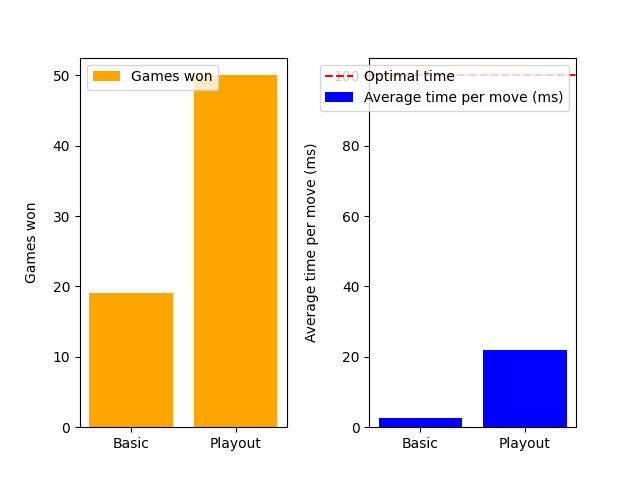
\includegraphics[width=0.8\textwidth]{../img/minimax_eval_closedworld.png}
  \caption{Comparison of number of wins and average time taken per ply of \texttt{basic} and \texttt{playout} evaluation functions in Minimax agent in the closed world}
  \label{minimaxCWEval}
\end{figure}

As shown in Figure \ref{minimaxCWEval}, the performance of two heuristic evaluation functions, namely \texttt{basic} and \texttt{playout}, is compared for a Minimax agent with a fixed \texttt{depth} of 3 and a fixed number of \texttt{samples} of 10 in a closed world environment. The left subplot presents the number of games won for the two evaluation functions, while the right subplot displays the average time taken to make a move. It can be observed that, similar to the open world setting, the playout heuristic outperforms the basic heuristic in terms of the number of games won, achieving more than twice as many wins as the basic heuristic. However, the playout heuristic is slower than the basic heuristic, as indicated by the right subplot. Despite this, the playout heuristic still performs within the optimal time range of 100ms, making it the preferred choice for the tournament. As a result, the Minimax agent will use the depth 9 and playout heuristic for the tournament.

In contrast to the open world setting, it is necessary to identify an appropriate value for the \texttt{samples} parameter in addition to the already-configured parameters in a closed world environment. Figure \ref{minimaxCWSamples} illustrates the experiment that was conducted to determine the optimal value for the \texttt{samples} parameter for the tournament. It indicates that the optimal value for the \texttt{samples} parameter is 30, as it results in the highest number of games won compared to the other tested values. This information can be used to determine the final parameter configuration for the Minimax agent. As a result, the Minimax agent will use the depth 3, playout heuristic and the samples 30 for the tournament.

\begin{figure}[h]
  \centering
  \captionsetup{justification=centering}
  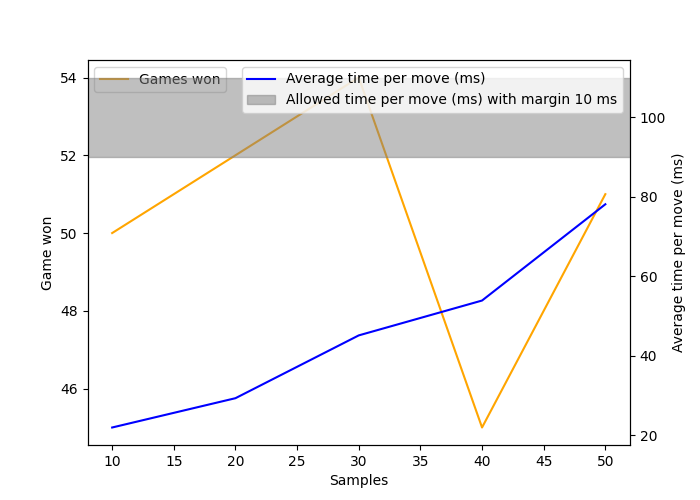
\includegraphics[width=0.8\textwidth]{../img/minimax_samples_closedworld.png}
  \caption{Comparison of number of wins and average time taken per ply of the \texttt{samples} value in Minimax agent in the closed world}
  \label{minimaxCWSamples}
\end{figure}




\subsection{Configuring MCTS Parameters}

To compare MCTS agents with other agents in an closed world environment tournament, it is necessary to determine the optimal values for the \texttt{limit}, \texttt{c}, \texttt{simulation} and \texttt{samples} parameters. As a starting point, the exploration constant was set to 1.41, which is generally considered an optimal value based on previous research \citep{AI4Ed}, the simulation parameter was set to \texttt{greedy} and the samples parameter was set to 10. With these parameters in place, an experiment involving 100 games was conducted to identify the optimal value for the limit parameter by testing various values for the number of iterations. The results of this experiment are shown in Figure \ref{mctsCWIterations}.

\begin{figure}[h]
  \centering
  \captionsetup{justification=centering}
  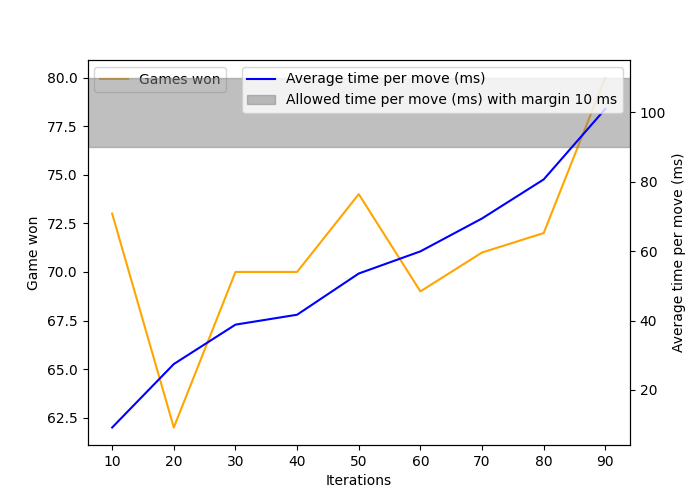
\includegraphics[width=0.8\textwidth]{../img/mcts_iterations_closedworld.png}
  \caption{Comparison of win rates and average time taken per ply of different fixed iterations in MCTS algorithm in the closed world}
  \label{mctsCWIterations}
\end{figure}

Similar to the Minimax agent, it can be seen that an increase in the number of \texttt{iterations} generally results in a corresponding increase in the average time taken per move, as well as an increase in the win rate. However, it is not clear why the number of games won using the value 10 for the iterations parameter is higher than the result of value of 20. This observation warrants further investigation in order to understand the underlying cause. By examining the shaded region in Figure \ref{mctsCWIterations}, which represents the optimal time per move, it can be determined that the optimal value for the \texttt{iterations} parameter is 90 in the closed world. This value results in a relatively high win rate and the lowest average time taken per move.

With the \texttt{iterations} parameter set to 90, the \texttt{simulation} value remaining at greedy and \texttt{samples} value remaining at 10, a new experiment was conducted to determine the optimal value for the \texttt{c}, exploration parameter, in MCTS. The results of this experiment are shown in Figure \ref{mctsCWC}. From the figure, it can be observed that the optimal value for the \texttt{c} parameter is 1.00, as it yields the highest number of wins while still operating within the optimal average time per move.

\begin{figure}[h]
  \centering
  \captionsetup{justification=centering}
  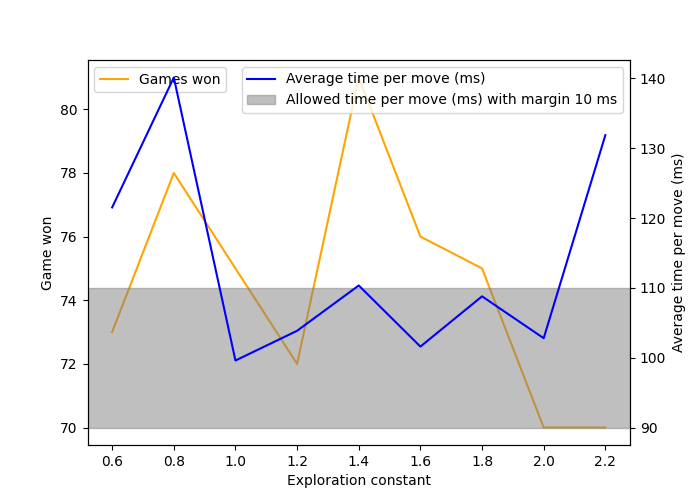
\includegraphics[width=0.8\textwidth]{../img/mcts_c_closedworld.png}
  \caption{Comparison of number of wins and average time taken per ply of different fixed exploration parameters in MCTS algorithm in the closed world}
  \label{mctsCWC}
\end{figure}

Like in the comparison of heuristic evaluation functions for the Minimax agent, bar plots were used to visualize the number of games won and average times per move for different simulation types in the MCTS algorithm. The left subplot in Figure \ref{mctsOWSimulations} compares the number of games won of the two simulations, and it can be seen that the greedy simulation performs significantly better than the random playouts. Additionally, the greedy simulation is much faster than the random playouts, as can be seen in the right subplot. This is due to the nature of random simulation, as discussed in Section \ref{MCTS}. Based on these results, we can conclude that the optimal parameters for the simulation in MCTS are greedy.

%\begin{figure}[h]
%  \centering
%  \captionsetup{justification=centering}
 % 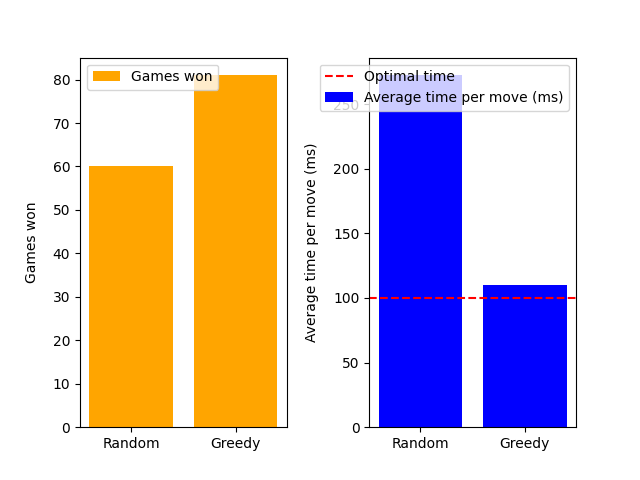
\includegraphics[width=0.8\textwidth]{../img/mcts_simulation_closedworld.png}
 % \caption{Comparison of number of games won and average time taken per ply of \texttt{random} and \texttt{greedy} simulations in MCTS algorithm in the closed world}
%  \label{mctsCWSimulations}
%\end{figure}

The results of the experiment conducted to determine the optimal value of the \texttt{samples} parameter for the MCTS agent in the closed-world tournament are shown in Figure 2. It can be seen that the highest number of games won is achieved with a samples value of 30. Based on these results, the MCTS agent will be configured with a limit of 100, an exploration constant of 1.41, a greedy simulation type, and a samples value of 30 for the closed-world tournament.

%\begin{figure}[h]
 % \centering
 % \captionsetup{justification=centering}
%  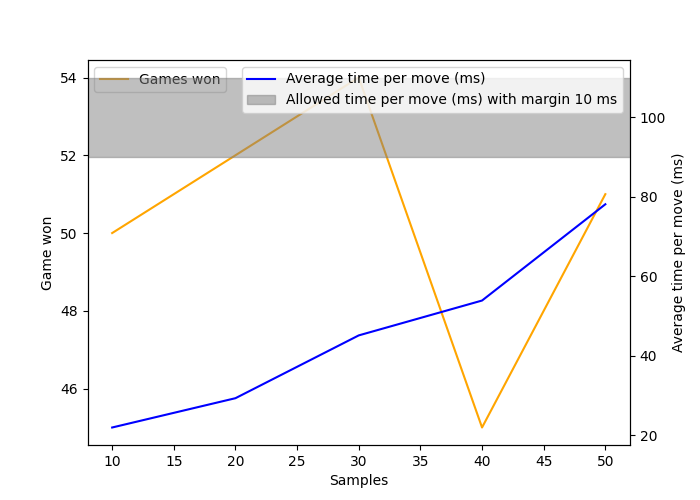
\includegraphics[width=0.8\textwidth]{../img/minimax_samples_closedworld.png}
 % \caption{Comparison of number of wins and average time taken per ply of the \texttt{samples} value in Minimax agent in the closed world}
 % \label{mctsCWSamples}
%\end{figure}
